\documentclass{article}\usepackage[]{graphicx}\usepackage[]{color}
%% maxwidth is the original width if it is less than linewidth
%% otherwise use linewidth (to make sure the graphics do not exceed the margin)
\makeatletter
\def\maxwidth{ %
  \ifdim\Gin@nat@width>\linewidth
    \linewidth
  \else
    \Gin@nat@width
  \fi
}
\makeatother

\definecolor{fgcolor}{rgb}{0.345, 0.345, 0.345}
\newcommand{\hlnum}[1]{\textcolor[rgb]{0.686,0.059,0.569}{#1}}%
\newcommand{\hlstr}[1]{\textcolor[rgb]{0.192,0.494,0.8}{#1}}%
\newcommand{\hlcom}[1]{\textcolor[rgb]{0.678,0.584,0.686}{\textit{#1}}}%
\newcommand{\hlopt}[1]{\textcolor[rgb]{0,0,0}{#1}}%
\newcommand{\hlstd}[1]{\textcolor[rgb]{0.345,0.345,0.345}{#1}}%
\newcommand{\hlkwa}[1]{\textcolor[rgb]{0.161,0.373,0.58}{\textbf{#1}}}%
\newcommand{\hlkwb}[1]{\textcolor[rgb]{0.69,0.353,0.396}{#1}}%
\newcommand{\hlkwc}[1]{\textcolor[rgb]{0.333,0.667,0.333}{#1}}%
\newcommand{\hlkwd}[1]{\textcolor[rgb]{0.737,0.353,0.396}{\textbf{#1}}}%

\usepackage{framed}
\makeatletter
\newenvironment{kframe}{%
 \def\at@end@of@kframe{}%
 \ifinner\ifhmode%
  \def\at@end@of@kframe{\end{minipage}}%
  \begin{minipage}{\columnwidth}%
 \fi\fi%
 \def\FrameCommand##1{\hskip\@totalleftmargin \hskip-\fboxsep
 \colorbox{shadecolor}{##1}\hskip-\fboxsep
     % There is no \\@totalrightmargin, so:
     \hskip-\linewidth \hskip-\@totalleftmargin \hskip\columnwidth}%
 \MakeFramed {\advance\hsize-\width
   \@totalleftmargin\z@ \linewidth\hsize
   \@setminipage}}%
 {\par\unskip\endMakeFramed%
 \at@end@of@kframe}
\makeatother

\definecolor{shadecolor}{rgb}{.97, .97, .97}
\definecolor{messagecolor}{rgb}{0, 0, 0}
\definecolor{warningcolor}{rgb}{1, 0, 1}
\definecolor{errorcolor}{rgb}{1, 0, 0}
\newenvironment{knitrout}{}{} % an empty environment to be redefined in TeX

\usepackage{alltt}
\usepackage{amscd, amssymb, amsmath, verbatim, setspace}
\usepackage[left=1.0in, right=1.0in, top=1.0in, bottom=1.0in]{geometry}
\usepackage{mathrsfs}
\usepackage{listings}


\IfFileExists{upquote.sty}{\usepackage{upquote}}{}
\begin{document}
\begin{flushright}
Arif Ali\\
Analytics 512 Statistical Learning\\
May 12, 2016\\
\end{flushright}

\begin{center}
\LARGE\textbf{Final Exam take home portion}
  \end{center}
\begin{knitrout}
\definecolor{shadecolor}{rgb}{0.969, 0.969, 0.969}\color{fgcolor}\begin{kframe}
\begin{alltt}
\hlkwd{library}\hlstd{(}\hlstr{"mlbench"}\hlstd{)}
\hlkwd{data}\hlstd{(Ozone)}
\end{alltt}
\end{kframe}
\end{knitrout}
\section*{Exercise 1}
\begin{knitrout}
\definecolor{shadecolor}{rgb}{0.969, 0.969, 0.969}\color{fgcolor}\begin{kframe}
\begin{alltt}
\hlkwd{names}\hlstd{(Ozone)} \hlkwb{<-} \hlkwd{c}\hlstd{(}\hlstr{"mo"}\hlstd{,}\hlstr{"day"}\hlstd{,}\hlstr{"wday"}\hlstd{,}\hlstr{"maxoz"}\hlstd{,}\hlstr{"pressh"}\hlstd{,}\hlstr{"wind"}\hlstd{,}\hlstr{"hum"}\hlstd{,}\hlstr{"temp1"}\hlstd{,}\hlstr{"temp2"}\hlstd{,}\hlstr{"inverh"}\hlstd{,}\hlstr{"pressg"}\hlstd{,}\hlstr{"invert"}\hlstd{,}\hlstr{"vis"}\hlstd{)}
\hlstd{Ozone}\hlopt{$}\hlstd{time} \hlkwb{=} \hlnum{1}\hlopt{:}\hlnum{366}
\hlstd{Ozone} \hlkwb{=} \hlkwd{na.omit}\hlstd{(Ozone)}
\hlstd{train} \hlkwb{=} \hlkwd{sample}\hlstd{(}\hlkwd{nrow}\hlstd{(Ozone),} \hlkwd{nrow}\hlstd{(Ozone)}\hlopt{*}\hlnum{.70}\hlstd{)}
\hlstd{Ozone_train} \hlkwb{=} \hlstd{Ozone[train,]}
\end{alltt}
\end{kframe}
\end{knitrout}
\section*{Exercise 2}
\begin{knitrout}
\definecolor{shadecolor}{rgb}{0.969, 0.969, 0.969}\color{fgcolor}\begin{kframe}
\begin{alltt}
\hlkwd{library}\hlstd{(boot)}
\hlstd{poly.cv.error} \hlkwb{=} \hlkwd{c}\hlstd{()}
\hlstd{d} \hlkwb{=} \hlnum{1}\hlopt{:}\hlnum{10}
\hlkwa{for}\hlstd{(i} \hlkwa{in} \hlstd{d)\{}
  \hlstd{ozone_pm} \hlkwb{=} \hlkwd{glm}\hlstd{(maxoz}\hlopt{~}\hlkwd{poly}\hlstd{(time,i),} \hlkwc{data} \hlstd{= Ozone_train)}
  \hlstd{poly.cv.error[i]} \hlkwb{=} \hlkwd{cv.glm}\hlstd{(Ozone_train, ozone_pm,} \hlkwc{K} \hlstd{=} \hlnum{10}\hlstd{)}\hlopt{$}\hlstd{delta[}\hlnum{2}\hlstd{]}
\hlstd{\}}
\hlkwd{plot}\hlstd{(d,poly.cv.error,}\hlkwc{type}\hlstd{=}\hlstr{"b"}\hlstd{)}
\end{alltt}
\end{kframe}
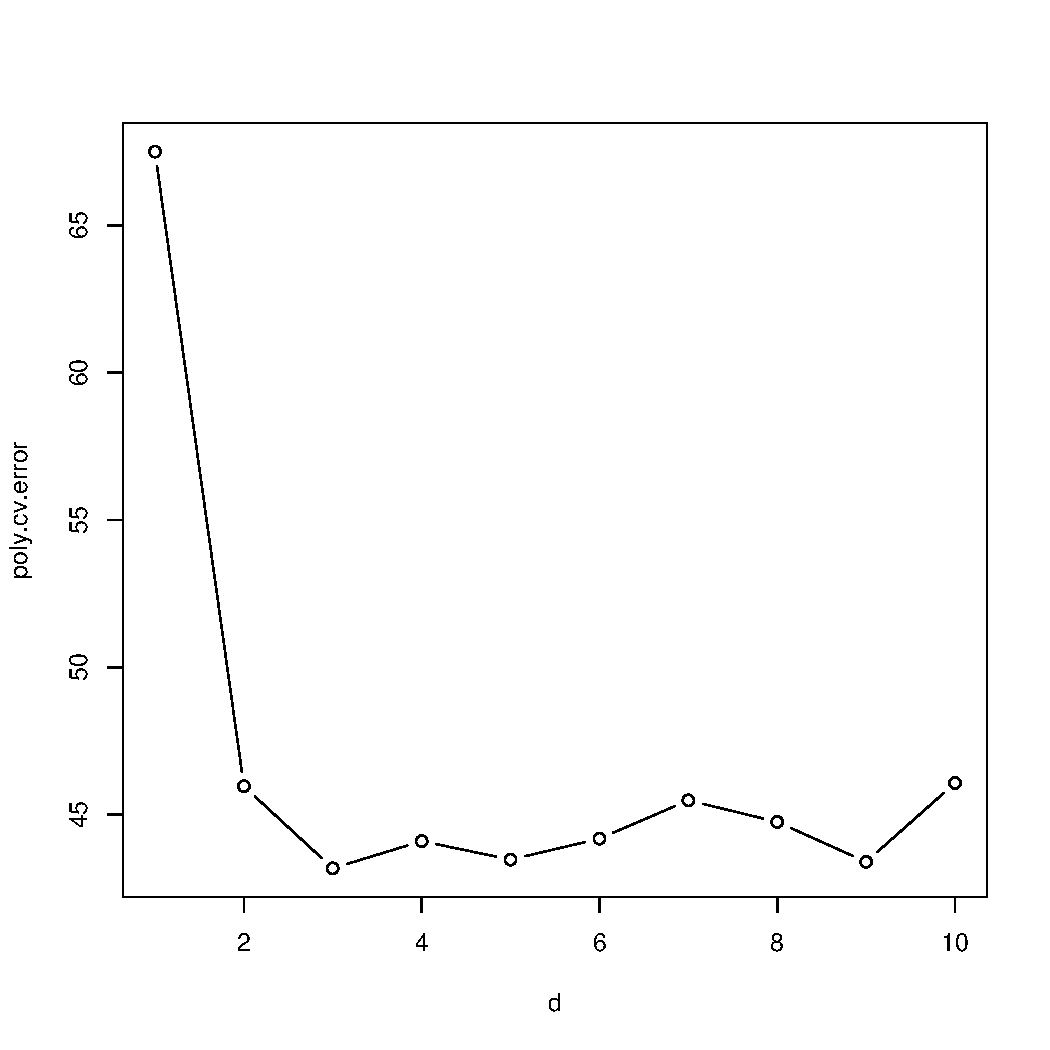
\includegraphics[width=0.50\linewidth]{figure/unnamed-chunk-4-1} 
\begin{kframe}\begin{alltt}
\hlstd{ozone_pm} \hlkwb{=} \hlkwd{glm}\hlstd{(maxoz}\hlopt{~}\hlkwd{poly}\hlstd{(time,d[poly.cv.error} \hlopt{==} \hlkwd{min}\hlstd{(poly.cv.error)]),} \hlkwc{data} \hlstd{= Ozone_train)}
\end{alltt}
\end{kframe}
\end{knitrout}

\end{document}
